\documentclass[twocolumn]{article}

\usepackage{amsmath,amssymb,amsfonts}
\usepackage{xcolor}
\usepackage{listings}
\usepackage{inputenc}
\usepackage{graphicx}
\usepackage{authblk}
\usepackage{enumerate}

\providecommand{\keywords}[1]
{
  \small	
  \textbf{\textit{Keywords---}} #1
}

\begin{document}
\author[1]{Eric Raphael Huiza Pereyra}
\affil[1]{Department of Postgraduate Studies, Pontifical Catholic University of Peru}
\affil[]{\textit{eric.huiza@pucp.edu.pe}}

\title{%
	\vspace{-2.0cm}
	\textbf{Talking with body expressions} \\	
	\Large \textbf{A Method for detecting sings in a weakly annotated dataset}
}

\maketitle
    
\begin{abstract}
People with deafness or hearing disabilities who aim to use computer based systems, state of art video classification and human action recognition rely in a combination of traditional and new methods like optical flow and 3D CNN. In this article we show a method to detect Peruvian Sign Language elements from a weakly annotated videos dataset. Video annotation techniques were applied increasing the models performance, as a result we achieved XX precision and XX exhaustiveness by training a 3D CNN with optical flow inputs.   \\
\keywords{video classification,human actions detection, optical flow, 3D CNN.}
\end{abstract}

\section{Introduction}\label{intro}

The World Health Organization (WHO) stated that 466 million people world wide have disabling hearing loss, estimating that by 2050 over 900 million people will have disabling hearing loss and will represent a global cost of 750.00 million dollars annually \cite{deafness_and_hearing_loss_2019}. 

The Peruvian Institute of Informatics and Statistics (INEI) executed a national disabilities survey with the objective to segment and better understand which disabilities affect the Peruvian population \cite{disabilities_survey_2012}, the results showed that 1.8\% of the Peruvian population present at least a partial or permanent deafness or hearing limitation. 

As of today it is completely viable to think about systems able to detect and transcribe signs languages. However, in the same way as spoken languages, signs languages also present local variations e.g. people that lives in the Lima metro area are not expect to use the same set of signs as people leaving in different parts of the country. Developing a dataset that describes the Peruvian Sign Language (PRL) \cite{lsp_2015} that can be used to train an AI model is expensive and difficult to achieve. 

The Pontifical Catholic University of Peru (PUCP) Grammar and  Signs research group created a PRL dataset \cite{lsp_dataset} that is weekly annotated because it does not show exactly the relation between the instant when a sign that is emitted and its corresponding translation.

This study was developed to obtain the Masters Degree in Informatics and Computer Science and proposes a novel Signs Detection Method (nSDm) that allows signs detection in a weakly annotated dataset and tries to answer the following questions:

\begin{enumerate}[(i)]
\item What are most relevant currently available techniques for training an AI model from  weakly annotated video and audio transcription?\label{q1}
\item How precise and exhaustive is the model described in the above question on the recognition of a reduced set of signs in a weakly annotated dataset?\label{q2}
\item What is the relation between the number of samples and the detection of new LSP elements in terms of nSDm precision and recall?\label{q3}
\end{enumerate}

nSDm will take advantage of the PRL dataset \cite{lsp_dataset} and will contribute with the generalization and progressive signs detection that could be used as a starting point for future studies including software accessibility improvements and human computer interaction for people with deafness and hearing limitations.

The rest of the article is organized as follows. In sec \ref{relatedwork} we review the related work on video classification and body actions recognition using both Optical Flow+Two Stream CNN and 3D CNN architectures. In sec \ref{method} we introduce nSDm and specify its architecture and design. In sec \ref{experimentation} we evaluate nSDm precision and recall and provide answers for the research questions \ref{q1},\ref{q2},\ref{q3}. In sec \ref{datasetdesc} we describe and provide the dataset details. In sec \ref{videoannot} we describe the video annotation and data pre-processing techniques applied to the dataset and finally in sec \ref{conclusion} we present our conclusion and describe future work.
\section{Related Work} \label{relatedwork}
\subsection{Action Recognition}
Human action recognition is a extensively studied field and available action recognition dataset: UCF101, HMDB51, THUMOS14  are available, researches tried to solve the human action recognition problem using different approaches including Optical Flow and 3D CNN \cite{qiu2017learning}.  \textbf{Optical Flow,} is defined as the pattern obtained from the motion of objects, surfaces and edges in a visual scene caused by the relative motion between the observer and a scene, it is achieved by distributing movement velocities and brightness across frames. It is a  key concept in action recognition from videos \cite{wang2019hallucinating}. Optical flow estimation is treated as an image reconstruction problem. Given a frame set, the optical flow is generated and allows to reconstruct one frame from the others \cite{zhu2018hidden}. Formally, taking the optical flow displacement field as input and training a CNN with it, then the network should have learned useful representations of the underlying motions. Even though Optical Flow represents the movement between a set of frames, if camera motion is considered as an action motion, it may corrupt the action classification \cite{wang2013dense}. Various types of camera motion can be observed in realistic videos, e.g., zooming, tilting, rotation, etc. \textbf{Motion Boundary Histogram (MBH),} It is a simple an efficient way to achieve robustness during human action detection when camera movements are mixed within the recorded actions by computing derivatives separately for the horizontal and vertical components of the optical flow. Since MBH represents the gradient of optical flow, locally constant camera motion is removed and information about changes in the flow field is kept. MBH is more robust to camera motion than optical flow, thus more discriminative for action recognition.\cite{wang2013dense}. 3D CNN are not as effective as optical flow to detect human actions on its own, 3D CNN can be trained to learn optical flow so we can avoid costly computation and storage and obtain task-specific motion representation  \cite{zhu2018hidden} and increase models performance, precision and exhaustiveness on human action recognition.
\subsection{Video Classification}
\textbf{Bag of Words.}
\\
\textbf{Fussing parallel CNN.}
\section{Method}\label{method}
\section{Experimentation}\label{experimentation}
\subsection{Dataset Description \cite{lsp_dataset}}\label{datasetdesc}
The LSP dataset was developed by the PUCP Grammar and Signs research group in 2014 and consists in a set of videos recorded during the interviews of 24 individuals, 12 male and 12 female informants, all of them are Lima Peru residents and reported to be borne with a permanent deafness condition or acquired the condition before the acquisition of Spanish. 

The dataset consists in 718 video clips recorded with a ADR-CX220 SONY HD camera which included an embedded microphone. The camera focused only the informant but also recorded questions, instructions and translations.

The video clips were recorded in three sessions with the following participants: A coordinator, a LSP \cite{lsp_2015} translator and a informant.\\

\textbf{Recording Session 1}: A 45-60 minutes semi structured interview that included: Biographic information as well as habits, anecdotes, opinion about cultural subjects and elicitation of names, states and actions. 

\textbf{Recording Session 2}: The informant was presented with a set of 55 cards describing actions and were asked to choose a set of them in order to build a coherent story that was subsequently told by the informant.

\textbf{Recording Session 3}: A LSP \cite{lsp_2015} conversation facilitated by the coordinator happening between the informant and the translator.\\

During all the sessions a LSP \cite{lsp_2015} translator performs a translation after a word or phrase is completed. The dataset is weakly annotated given there is not direct relation between the translation and the instant when the sign is emitted.

\subsection{Video Annotation}\label{videoannot}
\begin{figure}[ht!]
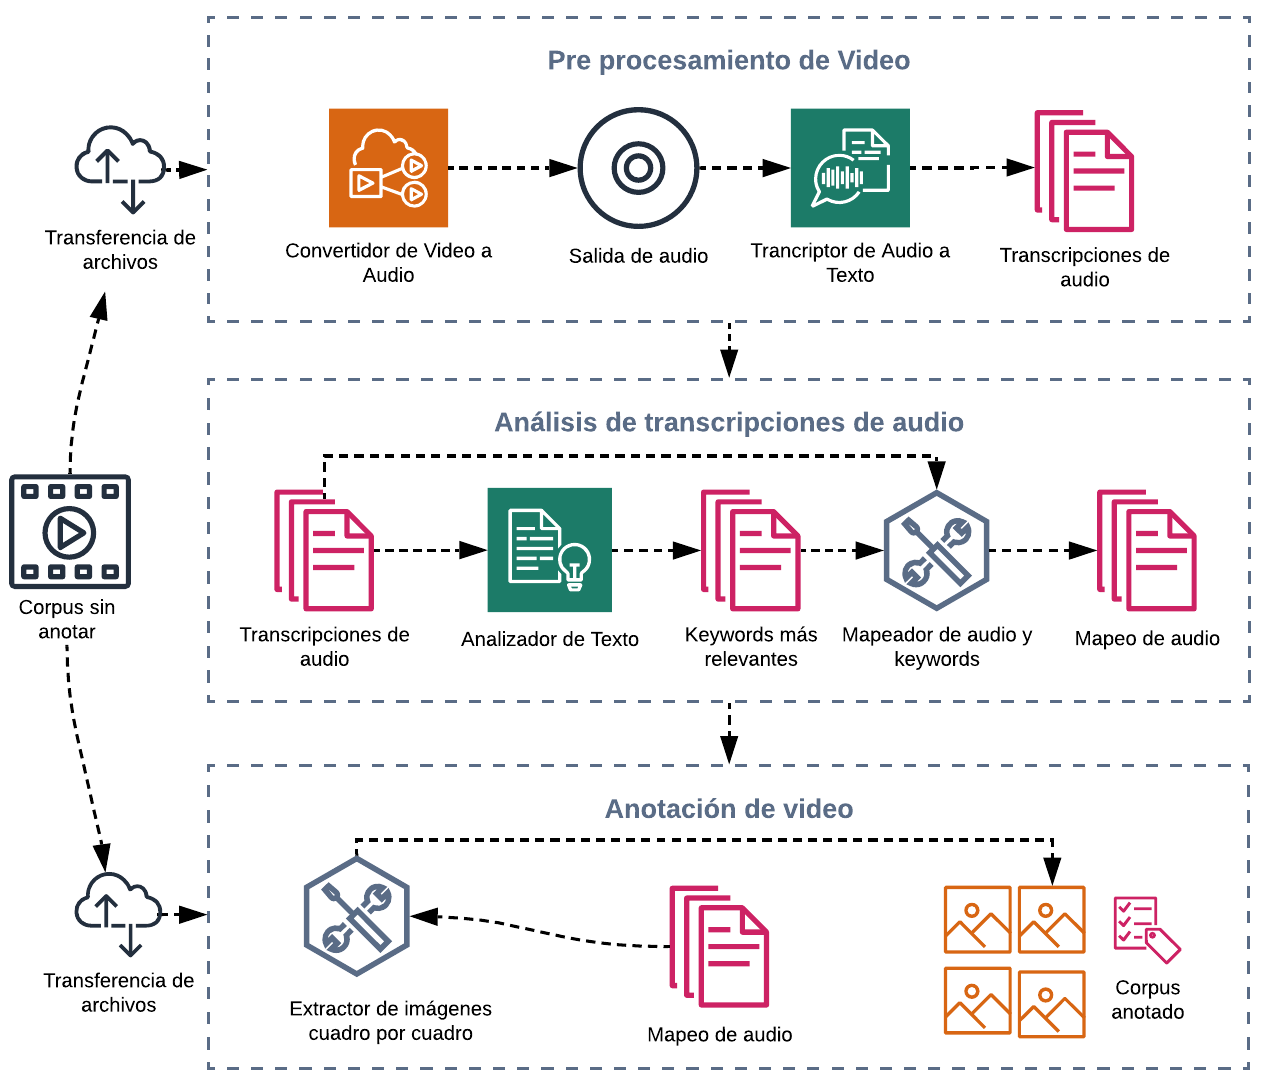
\includegraphics[width=\linewidth]{video-annotation-pipeline.png}
\caption{Video annotation process}
\end{figure}
\section{Conclusion}\label{conclusion}

\bibliographystyle{ieeetr}
\bibliography{References}


\end{document}
